\chapter{Mappings} \label{mappingchapter}

\section{Introduction}

A mapping is a relationship or transformation between models or
programs written in the same or different languages. Mappings are
a key part of the metamodelling process because of the important
role they play in describing how instances of one metamodel are to
be mapped to instances of other metamodels.

In the world of system development, mappings are everywhere:
between abstract (platform independent) models and platform
specific implementations, between legacy code and re-engineered
systems, across and within application and organisational domains.
Each of type of mappings places different requirements on the type
of mapping language that is required. Sometimes, a one shot,
unidirectional transformation is required. Other times, a mapping
must maintain consistency between models, perhaps by continuously
reconciling information about the state of both models. A mapping
language has to be able to deal with all these requirements.

At the time of writing, work is already underway, initiated by the
Object Management Group in the form of a request for proposals
(RFP) \cite{qvtrfp} to design a standard mapping language,
provisionally entitled QVT (Queries, Views, Transformations). Even
though there are many proposed meta-models for a mapping language
there are some basic foundations which are fairly independent of
the particular meta-model itself. This chapter begins with a
discussion on applications and existing technologies and
techniques for mappings and moves on to identify the requirements
for an ideal mapping language. Two languages, XMap and XSync are
then described that together address the complete requirements.

\section{Applications Of Mappings}

The application of mappings can be broadly divided into vertical,
horizontal and variant dimensions of a problem domain
\cite{mdatech}.

\subsection{Vertical Mappings}

Vertical mappings relate models and programs at different levels
of abstraction. Examples include mapping between a specification
and a design, and between a design and an implementation. In MDA
the mapping from more abstract models to less abstract, more
detailed models and programs is typically known as a PIM (platform
independent model) to PSM (platform specific model) mapping. Note,
these terms are somewhat relative (machine code can be viewed as
platform specific in relation to Java, yet Java is often viewed as
a platform specific in relation to UML).

The precise nature of a vertical PIM to PSM mapping will be
dependent upon the nature of the target platform. For example, the
following platform properties may be taken into account:

\begin{itemize}
\item Optimisation: improving one or more aspects of the efficiency
of the resultant platform specific code, e.g. efficiency of memory
usage, speed of execution, and usage of dynamic memory allocation.
\item Extensibility: generating platform specific code that
is more open to adaptation, e.g. through the use of polymorphic
interfaces.
\item Language paradigm: Removing (or adding) language features,
for instance substituting single inheritance for multi-inheritance
or removing inheritance altogether.
\item Architecture: if the target platform is a messaging broker,
such as CORBA, rules will be defined for realising the platform
independent mapping in terms of appropriate interface calls to the
message broker.
\item Trustworthiness: visible and clear mappings may allow some
level of reasoning to be applied to the target notation, which may
enable certain properties (e.g. pertaining to safety) to be
automatically established.
\end{itemize}

It is important to note that vertical mappings may also go in the
reverse direction, e.g. from implementation to design. This is
particularly appropriate for reverse engineering. Here the essence
of the functionality of the platform specific language is reverse
engineered into another language. Typically, this process will not
be an automatic one, but must be supported by tools.

\subsection{Horizontal Mappings}

Whilst vertical mappings have received much attention in the MDA
literature, horizontal mappings are just as important. Horizontal
mappings describe relationships between different views of a
problem domain. Examples of these include:

\subsubsection{System Views}

In large systems, many different aspects of the problem domain
will need to be integrated. This may include different aspects of
the business domain such as marketing or sales, or the technology
domain such as safety or security. Critically, many of these
different aspects will overlap. Horizontal mappings can be defined
between languages that capture these different views, allowing
them to be consistently managed.

\subsubsection{Language Views}

Complex systems can rarely be modelled using a single notation. As
the popularity of UML has demonstrated, different notations are
required to precisely and succinctly model different view points
of the system. For instance, in UML, class diagrams are used to
model the static structure of a system and a completely different
language, state machines for example, to model the dynamic view
point. Even though these notations are different they describe the
same system with overlapping views and hence there exists a
relationship between them.

As shown in chapter \ref{concretechapter}, horizontal mappings
provide a means of integrating language notations in a way that
ensures changes in one view automatically updates other views.
Figure \ref{horizontalmap} shows how this might work for a small
part of UML. Here, it is assumed that there is a core OO modelling
language, with its own, precisely defined semantics. Many of the
different modelling notations provided by UML are modelled as a
view on the underlying OO modelling language. Mappings reconcile
changes to the diagrams by making changes to the underlying OO
model, which in turn may impact models in other diagrams.

\begin{figure}[htb]
\begin{center}
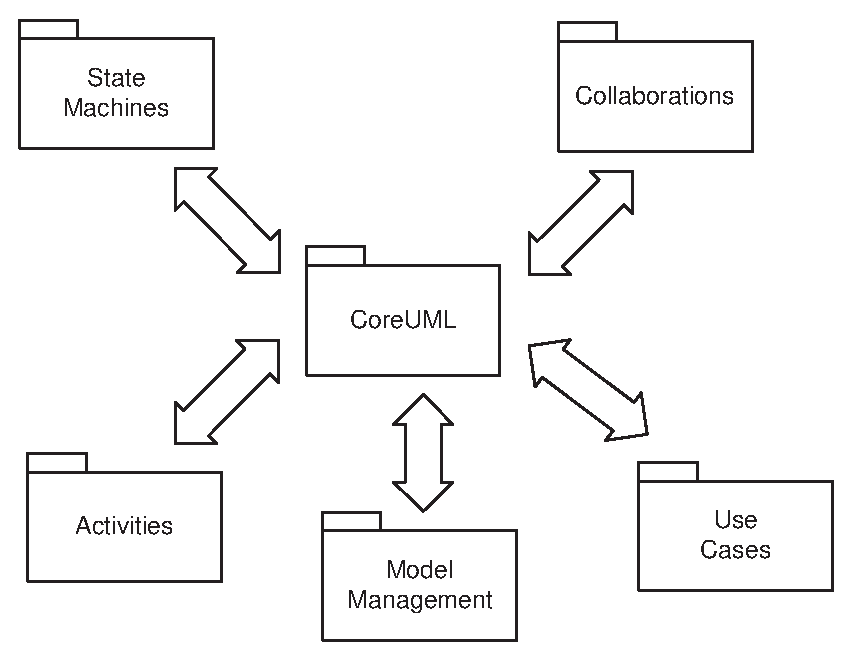
\includegraphics[width=10cm]{Mappings/figures/HorizontalMapExample}
\caption{An example of a horizontal mapping between core UML and
its diagrams} \label{horizontalmap}
\end{center}
\end{figure}

Of course, previous chapters have shown that horizontal mappings
are also necessary for integrating different aspects of a
modelling language. Mappings between concrete syntax and abstract
syntax, and between abstract syntax and a semantic domain are all
critical parts of a language definition.

\subsection{Variant Dimensions}

Variant dimensions include product families and product
configurations. Mappings can model the relationship between
variant dimensions enabling each dimension to be precisely related
to one another.

\section{Types of Mappings}

\subsection{Unidirectional Mappings}

Unidirectional mappings take an input model or collection of input
models and generate an output model in one go. A unidirectional
mapping may record information about the relationship between the
input and output model, but there is no dependency of the input
model on the output model. If the input model/s change, then the
entire mapping must be rerun again in order to re-generate the
output model.

An example of a one shot mapping is a code generator, that takes a
platform independent model as its input, and generates a platform
specific model or program.

\subsection{Synchronised Mappings}

Synchronised mappings are a special class of mapping where it is
important to continuously manage consistent relationships between
models. This requirement can occur in many different situations.
One common example is maintaining consistency between a model and
the code that it is being transformed to. This would be a
requirement if a programmer wants to add/change code whilst
maintaining consistency with the model it is generated from. In
this scenario a change to the code would be immediately reflected
back in the model, and vice versa: if the model was changed, it
would be reflected in changes in the code. In the context of
horizontal mappings, synchronised mappings have an important part
to play in maintaining consistency between different viewpoints on
a model.

\section{Requirements of a Mapping Language}

When applying mappings on real projects it becomes apparent that
there are some key requirements that a mapping language must
support if it is to be of practical use. These include the
following:

\begin{itemize}
\item Support for mappings of relatively high complexity. For
example, the mapping language should be able to model complex
mappings, such as transforming an object oriented model into a
relational model including the mapping of the same attribute to
different columns for foreign key membership \cite{qvtrfp}. In
practice, this means that the mapping language must provide good
support for arbitrarily complex queries of models (to be able to
access the information necessary to drive a complex mapping), and
support the ability to modify models  using relatively low level
operations (such operations can, if used sensibly, significantly
reduce the size and complexity of a mapping).

\item Support for reuse. It should be possible to extend and adapt
mappings with ease. This meets the need to be able to reuse
existing mappings rather than having to create them from scratch
each time.

\item Facilitate the merging of models. If the source metamodel of
a mapping represents a graph then any duplicate elements that are
generated by the mapping must be merged.

\item Provide mechanisms that support the structuring of mappings, e.g.
being able to model the fact that a mapping owns or is dependent
on sub-mappings.

\item Be able to record information about a mapping to provide
traceability during the mapping process.

\item Integration within the metamodel architecture, so that
mappings may access models at all levels.

\item Support for execution. It may seem obvious, but a mapping
should be executable in order to support the physical generation
of new models from a mapping. This is contrasted with a
non-executable mapping (see below).

\item Provide diagrammatic notations that can be used to visualize
mappings. Visual models have an important role to play in
communicating the overall purpose of a mapping.

\item Support for bi-directional and persistent mappings. As described
above, this is essential in being able to support mappings where
models must be synchronised with other models.

\item Support for mapping specifications. A mapping specification
is a non-executable description of `what' a mapping does, which
does not commit to`how' the mapping will be implemented. Mapping
specifications are a valuable means of validating the correctness
of an executable mapping, or as a contract between a designer and
an implementor.
\end{itemize}

An important question to ask at this point is whether all these
requirements can be addressed by a single mapping language. In our
experience, it does not make sense to have a 'one size fits all'
mapping language because not all the requirements are
complimentary. In particular, there is a strong distinction to be
made between a bi-directional and unidirectional mapping
languages. Each are likely to be targeted at different types of
problems and thus have different requirements in terms of
expressibility and efficiency.

Instead, it is better to use a small number of mapping languages,
each targeted at a specific mapping capability, yet still capable
of being combined within a single model. This is strategy taken in
this book. In the following sections, two mapping languages, XMap
and XSync are described each aimed at addressing complimentary
mapping capabilities.

\section{XMap}

XMap is a language designed to support unidirectional mappings. It
includes the following features:

\begin{description}
\item [Mappings] Mapping are the used to model unidirectional
transformations from source to target values. Mappings have state
and can be associated with other mappings. \item[Syntax] Mappings
have a visual syntax, enabling them to be drawn between model
elements in a class diagram, and a concrete syntax for describing
the detailed aspects of the mapping. \item[Executability] Mappings
have an operational semantics enabling them to be used to
transform large models. \item[Patterns] Mappings are described in
terms of patterns. A pattern describes what a mapping does in
terms of how a value in the source model is related to a value in
the target model - this provides maximum declarative
expressibility, whilst also remaining executable. Patterns are
described in a pattern language that runs over OCL expressions.
\item[OCL] Mappings can make use of OCL to express complex model
navigations.
\end{description}

In addition, XMap provides {\em Mapping specifications}. These are
multi-directional, non-executable, transformation specifications.
In the general case they are non-executable, but useful restricted
types of mapping specification can be automatically refined into
mappings. Mapping specifications are written in a constraint
language, in this case OCL. Typically they are used in the
specification stages of system development.

The syntax and semantics of XMap are described in exactly the same
way that all languages are defined in XMF: as an XMF metamodel,
with an operational semantics expressed in terms of XOCL.

\section{XMap Syntax}

XMap has a visual syntax and a textual syntax. As shown in figure
\ref{examplemapping} the visual syntax consists of a mapping arrow
that can be associated with other model elements such as classes
in a class diagram. A mapping has a collection of domain or input
elements that are associated with the tail of the arrow, and a
single range or output element that is associated with the end of
the arrow.

\begin{figure}[htb]
\begin{center}
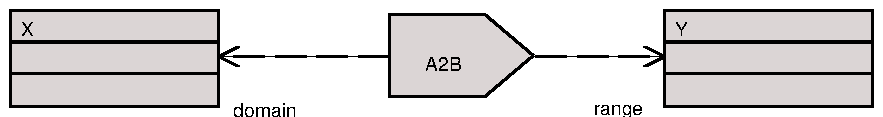
\includegraphics[width=11cm]{Mappings/figures/mapping.pdf}
\caption{An example mapping} \label{examplemapping}
\end{center}
\end{figure}


The textual syntax of a mapping consists of a mapping declaration,
which is equivalent to a mapping arrow on a diagram:

\begin{lstlisting}
@Map <name>(<domain_1>,<domain_2>,...<domain_n>)-><range>

end
\end{lstlisting}\noindent A mapping contains a collection of clauses of the form:

\begin{lstlisting}
@Clause <name>
  <pattern>
end
\end{lstlisting}\noindent Note, each clause must have a different name.

A pattern is the mechanism that is used to match values in the
domain of the mapping to values in the range. It has the general
form:

\begin{lstlisting}
<exp> do
  <exp>
where
  <exp>
\end{lstlisting}Expressions are written in a mixture of XOCL expressions and
patterns expressions, where a pattern expression is a syntactical
relationship between expressions containing variables that are
bound by pattern matching. A common pattern used in mappings is to
relate object constructors. These describe a pattern match between
a domain object constructor and a range object constructor subject
to there being a pattern match between slot value expressions. An
example of this is:

\begin{lstlisting}
X[a = A] do
  Y [b = A]
\end{lstlisting}
Here the variable, A, is bound to the value of the slot a of any
instance of the class X using the expression a = A. This value is
then matched with the value of the slot b. The result of this
expression will be to match any instance of the class X with the
class Y, subject to the value of the slot b being equal to the
value of a.

Patterns can contain arbitrarily complex expressions. For
instance, this expression matches a with another constructor,
which contains a variable c, which is then matched with b:


\begin{lstlisting}
X[a =
  Z[c = A]] do
  Y [b = A]
\end{lstlisting}\noindent Patterns may also be embedded in sets and sequences:

\begin{lstlisting}
X[a =
  Set{Z[c = A]]} do
  Y [b = A]
\end{lstlisting}In this case, the slot a must be an instance of an attribute of
type Set(Z) and provided it contains an single instances of Z will
be matched.

Patterns can also be used in a very implicit fashion, to state
properties of values that must match. For instance, consider the
requirement to match a with an object belonging to a set, subject
to a slot being of a specific value. This could be expressed as
follows:

\begin{lstlisting}
X[a = S->including(Z[c = 1,d = A]]) do
  Y [b = A]
\end{lstlisting}This will match an object belonging to the set a subject to its
slot c being equal to 1. The value of S will be the remaining
elements of the set.

The 'where' component of a clause can be used to write additional
conditions on the pattern. Consider the following pattern, in
which the relationship between the variables A and B are related
by a {\tt where} expression:

\begin{lstlisting}
X[a = A]] do
  Y [b = B]
  where B = A + 1
\end{lstlisting}Finally, a mapping clause may call other mappings. This is
achieved by creating an instances of the mapping, and passing it
the appropriate domain values:

\begin{lstlisting}
X[a = A]] do
  Y [b = B]
  where B = mapIt(A)
\end{lstlisting}Here, the value of B is assigned the result of passing the value
of A to the mapping called mapIt. Note that a mapping can also be
instantiated and then invoked. This enables values to be passed to
the mapping via its constructor, e.g. mapIt(5)(A).

Finally, it is common to iterate over a collection of values,
mapping each one in turn. This type of mapping would look like so:

\begin{lstlisting}
X[a = A]] do
  Y [b = B]
  where B = A->collect(a | mapIt()(a))
\end{lstlisting}\noindent This would pass each element of A into the mapIt()
mapping collecting together all their values and assigning them to
B.

\section{XMap Examples}

This section demonstrates two mappings written using XMap: a
mapping from StateMachines to Java and a mapping from Java to XML.
Together they aim to demonstrate the main features of XMap and to
give an understanding of the essential requirements of a mapping
language.

\subsection{StateMachines to Java}

The purpose of this mapping is to translate a StateMachine into a
Java class. The source of the mapping is the StateMachines
metamodel described in chapter \ref{abschapter} and the class
diagram for this metamodel is repeated below.

\begin{figure}[htb]
\begin{center}
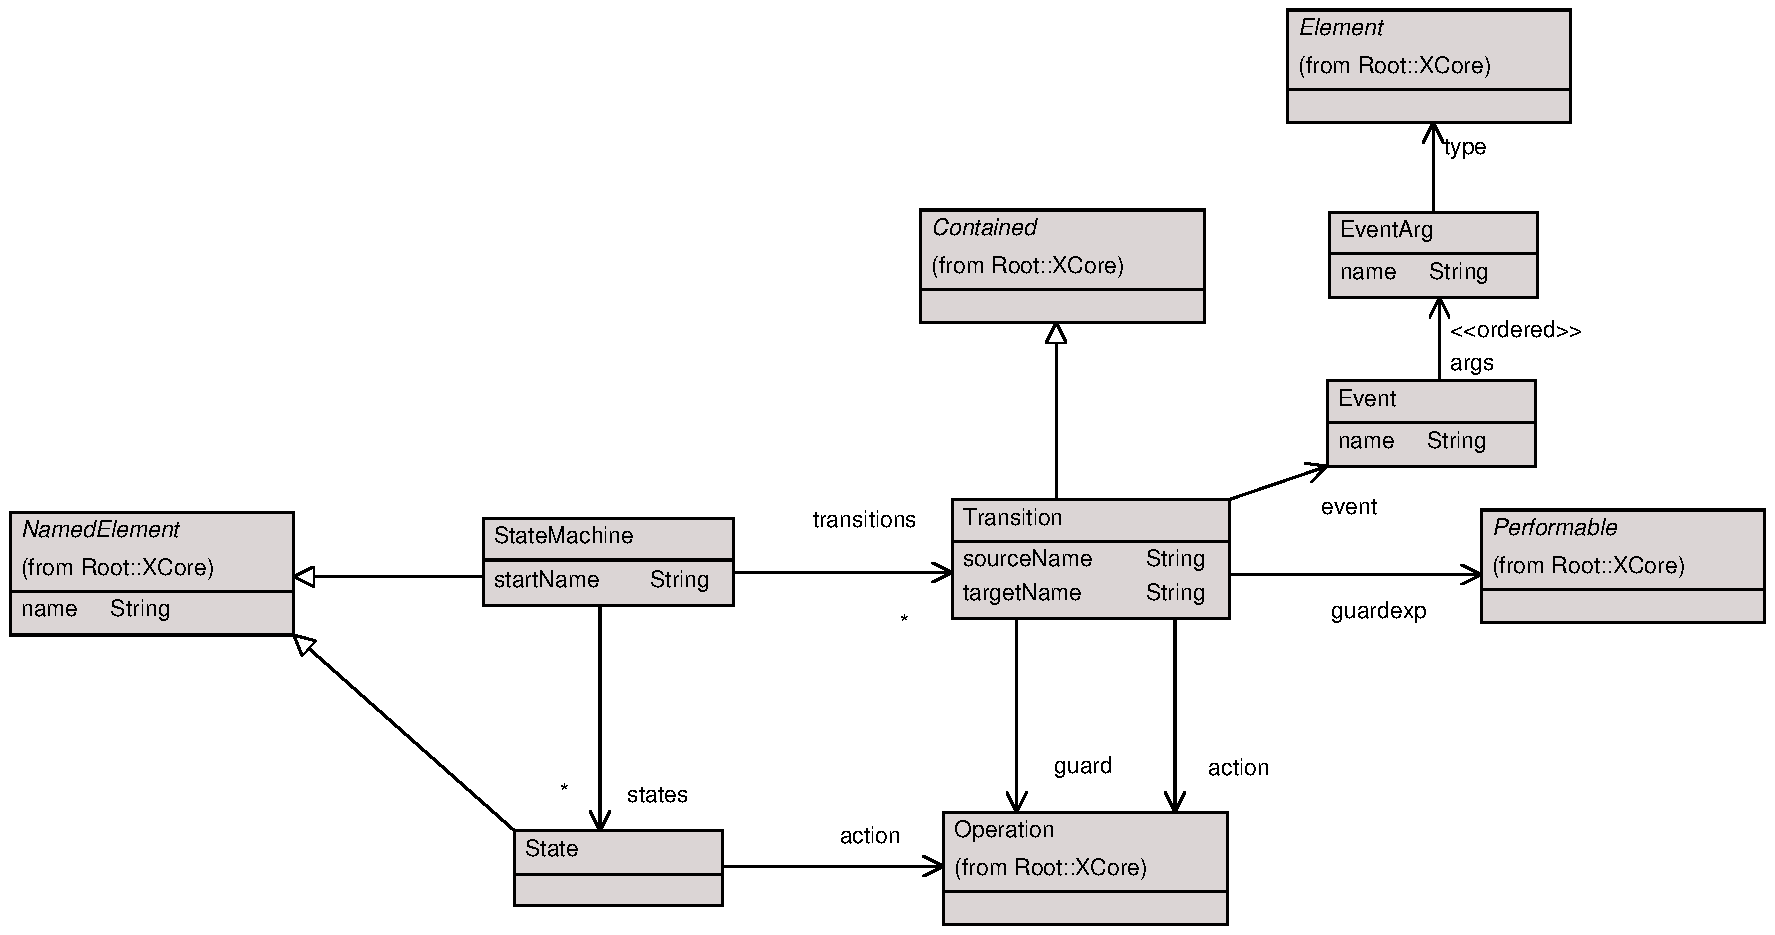
\includegraphics[width=17cm]{Mappings/figures/SMAbs2.pdf}
\caption{The abstract syntax metamodel for StateMachines}
\end{center}
\end{figure}

The target of the mapping is a simple model of Java as shown in
figure \ref{javamodel}. A Java program is a collection of named
classes. A Java class has a collection of member properties, which
may be named fields (attributes) or methods. A method has a name,
a body and  a return type and a sequence of arguments that have a
name and a type.

\begin{figure}[htb]
\begin{center}
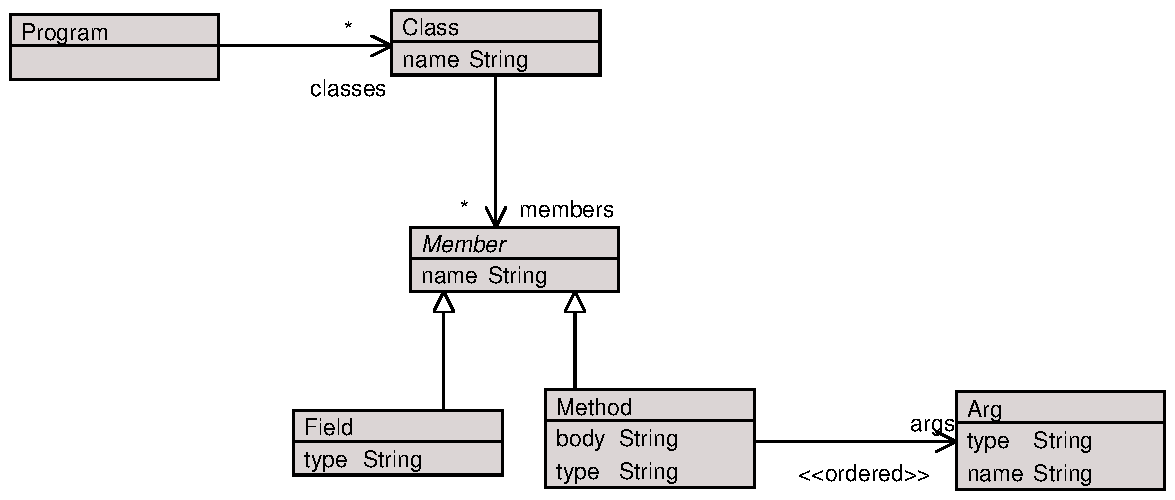
\includegraphics[width=15cm]{Mappings/figures/javamodel.pdf}
\caption{The abstract syntax metamodel for Java} \label{javamodel}
\end{center}
\end{figure}

The mapping is shown in figure \ref{javamapping}. It maps a
StateMachine into a Java class with an attribute called state and
maps each transition to a method that changes the value of state
from the source state to the target state.

\begin{figure}[htb]
\begin{center}
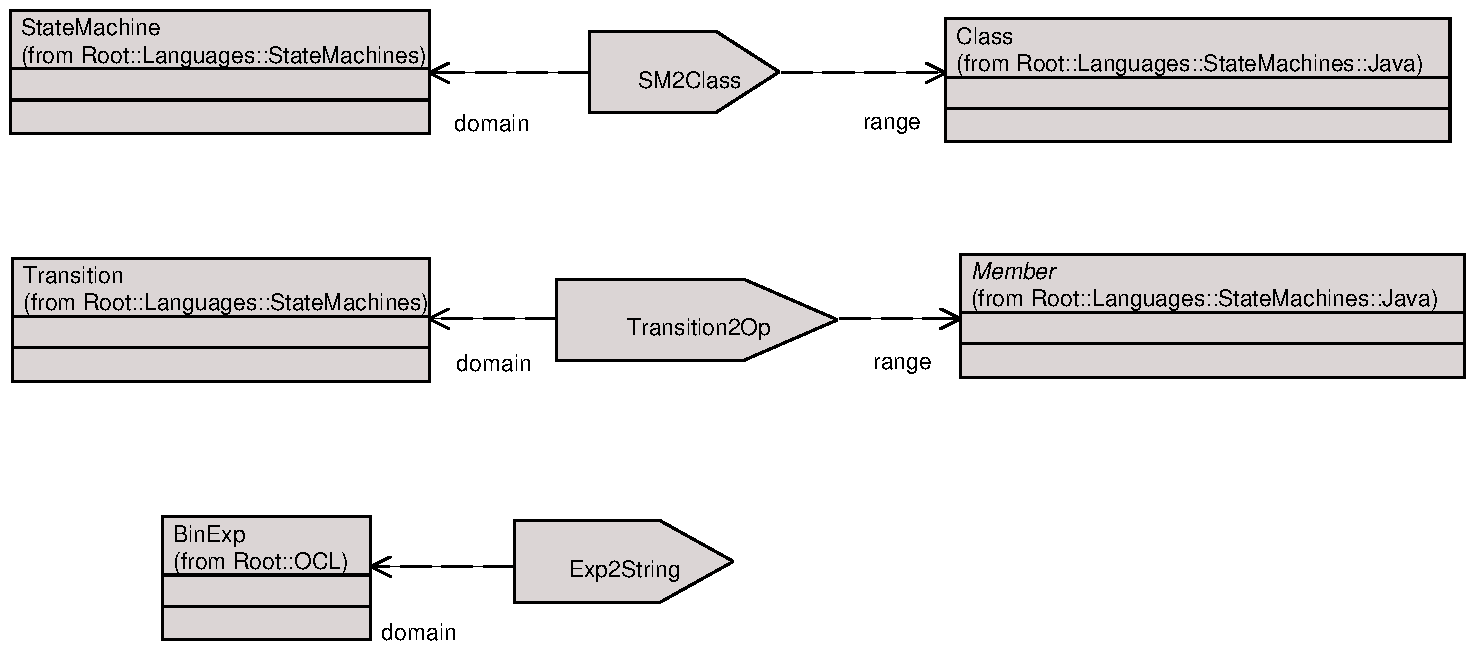
\includegraphics[width=15cm]{Mappings/figures/javamapping.pdf}
\caption{The StateMachine to Java mapping} \label{javamapping}
\end{center}
\end{figure}

The detail of the StateMachine mapping are described by the
following code. A mapping consists of a collection of clauses,
which are pattern matches between patterns of source and target
objects. Whenever a collection of source values is successfully
matched to the input of the mapping, the resulting collection of
values after the do expression is generated. Variables can be used
within clauses, and matched against values of slots in objects.
Because XMap builds on XOCL, XOCL expressions can also be used to
capture complex relationships between variables.


\begin{lstlisting}
@Map SM2Class(StateMachines::StateMachine)->Java::Class
  @Clause ToClass
    s = StateMachine
      [name = N,
       transitions = T,
       states = S] do
    Class
      [name = N,
       members = M->including(
         Field
           [name = "state",
            type = "String" ])]
    where M = T->collect(t | Transition2Method(t))
  end
\end{lstlisting}
In this example, whenever the mapping is given a StateMachine
object with a name equal to the variable N, a set of transitions T
and a set of states S, it will generate an instance of the class
Java::Class. This will have a name equal to N and members that
includes a single state attribute named "state" and a set of
methods, M. The where clause is used to calculate the value M. It
matches M with the results of iterating over the transitions, T,
and applying the Transition2Method mapping.

\noindent The mapping from transitions to Java methods is shown
below:


\begin{lstlisting}
  @Map Transition2Method(Transition)->Java::Method
    @Clause Transition2Method
      t = Transition
        [event = Event[name = N] ] do
      Method
        [name = N,
         body = B]
      where
        B = "if (" + Exp2String()(t.guardexp.performable) + ")\n" +
        "  this.state := " + "\"" + t.targetName + "\"" + "; \n"

    end
  end
\end{lstlisting}
This mapping matches a Transition owning an Event named N to a
Java Method with a name N and a body B. This mapping illustrates
how patterns can capture arbitrarily nested structures: any depth
of object structure could have been captured by the expression.

The definition of the body, B, requires some explanation. Because
the mapping generates a textual body, this expression constructs a
string. The string contains an "if" expression whose guard is the
result of mapping the transition's guard expression (an instances
of the OCL metamodel) into a string (see below). The result of the
"if" expression is an assignment statement that assigns the state
variable to be the target of the transition.

\subsubsection{Mapping Guard Expressions}

Whilst the above mapping deals with the mapping to the
superstructure of Java, it does not deal with mapping the guards
and actions of the StateMachine. However, in order to be able to
{\em run} the Java, these will need mapping across too. As an
example, the following mapping describes how some sub-expressions
of OCL can be mapped into Java code.


\begin{lstlisting}
  @Map Exp2String(OCL::BinExp)->String
    @Clause BinExp2String
      BinExp
      [binOp = N,
       left = L,
       right = R] do
       self(L) + " " + N + " " + self(R)
    end
    @Clause IntExp2String
      IntExp
      [value = V] do
       V
    end
    @Clause Dot2String
      Dot
      [name = N,
       target = S] do
       if S->isKindOf(OCL::Self) then
         "self"
       else
         self(S)
       end + "." + N
    end
    @Clause BoolExp2String
      BoolExp
      [value = V] do
       V
    end
  end
\end{lstlisting}
This mapping contains a number of clauses, which are matched
against an sub-expression of OCL. In order to understand this
mapping, it is necessary to understand the OCL metamodel. The
relevant fragment of this is shown below in figure
\ref{oclfragment}.

\begin{figure}[htb]
\begin{center}
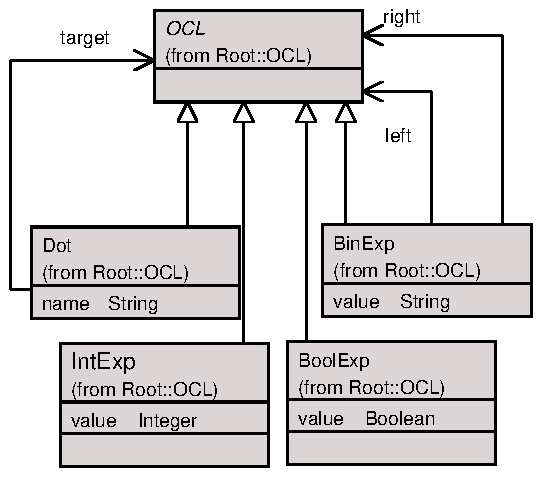
\includegraphics[width=7cm]{Mappings/figures/oclfragment.pdf}
\caption{Fragment of OCL expression metamodel} \label{oclfragment}
\end{center}
\end{figure}

The first clause of this expression matches against any binary
expression, and generates a string containing the results of
mapping the left hand expression followed by the binary operator
and the result of mapping the right hand expression. The following
clauses describe what should happen for integer expressions, dot
expressions and boolean expressions.

As an example, consider the StateMachine in figure
\ref{trafficlight}. The body of the guard on the GreenRed
transition will be parsed into an instance of an OCL expression.
The mapping described above will translate the transition and its
guard expression into the following Java code:

\begin{lstlisting}
public GreenRed() if (self.count < 10)
  this.state := "Red";
\end{lstlisting}\subsection{Mapping to XML}

This section gives an example of using XMap to map between Java
and XML. The aim of this example is to illustrate the ability of
mappings to record information about the execution of a mapping.

A model of XML is shown in figure \ref{xmlmodel}. An XML document
consists of a root node, which may be an element, or a text
string. Elements can have attributes, which have a name and a
value. Elements may also have child nodes.

\begin{figure}[htb]
\begin{center}
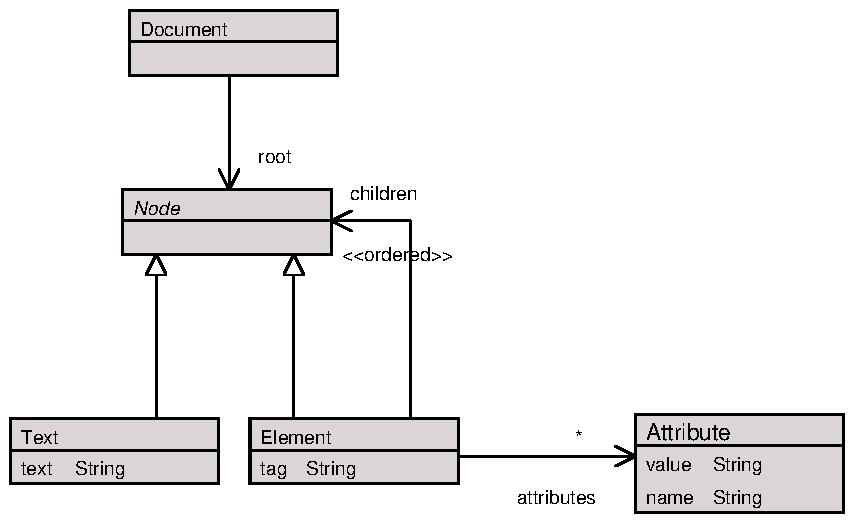
\includegraphics[width=11cm]{Mappings/figures/xmlmodel.pdf}
\caption{Abstract syntax model for XML} \label{xmlmodel}
\end{center}
\end{figure}

A mapping between Java and XML maps each element of the Java model
(classes, fields, methods and arguments into XML elements. The
relationship between XML elements and their children matches the
hierarchical relationship between the elements in the Java model.
The mapping diagram is shown in figure \ref{xmlmapping}.

\begin{figure}[htb]
\begin{center}
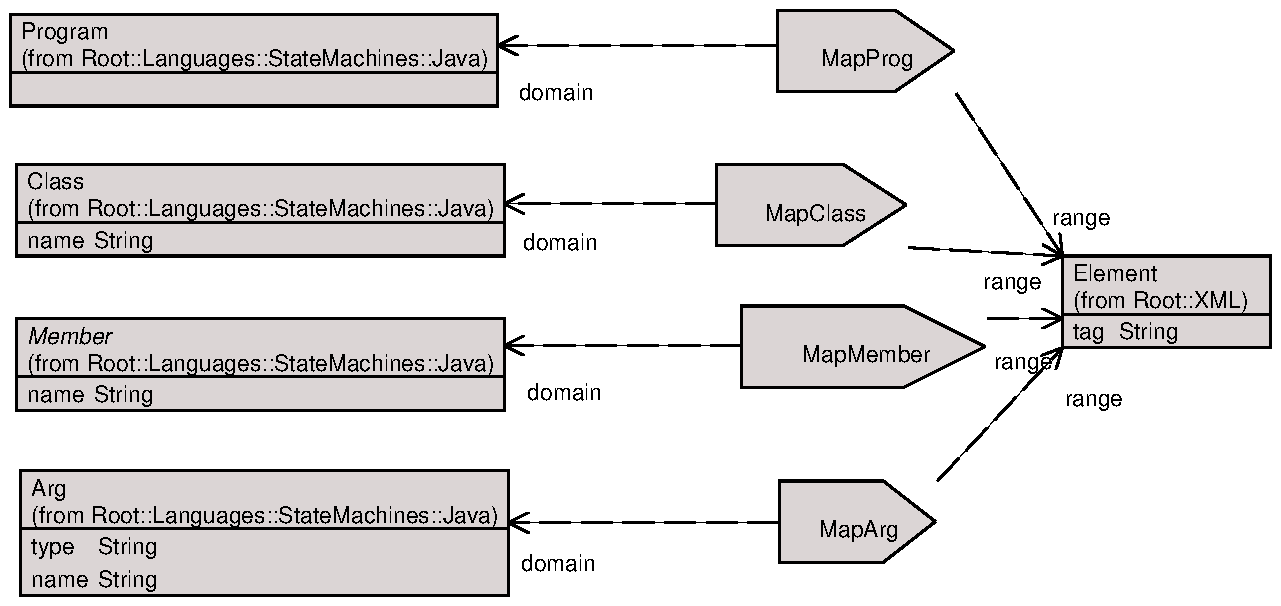
\includegraphics[width=14cm]{Mappings/figures/xmlmapping.pdf}
\caption{Mapping from Java to XML} \label{xmlmapping}
\end{center}
\end{figure}

The mapping from a Java program to an element is shown below. The
operation getId() will return an id ref for an element if that
element has already been generated, alternatively it will create a
new one and place it in a table. All subordinate mappings can
reach this mapping via their 'owner' slot.


\begin{lstlisting}
  @Map MapProg(Java::Program)->XML::Element

    @Attribute mapClass : MapClass = MapClass(self) end
    @Attribute idTable : Table = Table(100) end

    @Operation getId(name)

      if idTable.hasKey(name) then
        idTable.get(name)
      else
        idTable.put(name,"id" + idTable.keys()->size.toString());
        idTable.get(name)
      end
    end

    @Clause Program2Element
      Program
        [classes = C]
      do
      Element
        [tag = "Program",
         attributes = Set{},
         children = E]
      where
      E = C->collect(c | mapClass(c))
    end
  end
\end{lstlisting}
The mapping from classes to XML elements is more complicated. It
maps a class with name N and members M to an element tagged as a
"Class" containing two attributes. The first attribute corresponds
to the name attribute of the class, and thus has the name "name"
and value N. The second attribute provide an id for the element,
which is the result of running its getId() operation.


\begin{lstlisting}
@Map MapClass(Java::Class)->XML::Element

  @Attribute owner : MapProg end
  @Attribute mapMember : MapMember = MapMember(self) end

  @Constructor(owner) end

  @Operation getId(name)
    owner.getId(name)
  end

  @Clause Class2Element
    Class
      [name = N,
       members = M] do
    Element
      [tag = "Class",
        attributes =
          Set{}->including(
             Attribute
               [name = "name",
                value = N])->including(
                  Attribute
                    [name = "id",
                     value = self.getId(N)]),
         children = E]
      where
      E = M->collect(m | mapMember(m))
  end
end
\end{lstlisting}\noindent Exactly the same strategy is used to map Field, Methods
and Arguments to XML Elements. The following shows the mapping for
Fields:


\begin{lstlisting}
@Map MapMember(Java::Member)->XML::Element

  @Attribute owner : MapClass end
  @Attribute mapArg : MapArg = MapArg(self) end

  @Constructor(owner) end

  @Operation getId(name)
    owner.getId(name)
  end

  @Clause Field2Element
    Java::Field
      [name = N,
      type = T] do
    Element
      [tag = "Field",
         attributes =
           Set{}->including(
             Attribute
               [name = "name",
                value = N])->including(
                  Attribute
                    [name = "type",
                     value = self.getId(T)]),
      children = Set{}]
  end
end
\end{lstlisting}
\section{Mapping Specifications}

A mapping specification is useful in describing what a mapping
does as opposed to how it is to be implemented. Mapping
specifications do not require any additional modelling facilities
beyond OCL. As shown in figure \ref{mappingspec}, a mapping
specification consists of a number of mapping classes, which sit
between the elements of the models that are to be mapped.

\begin{figure}[htb]
\begin{center}
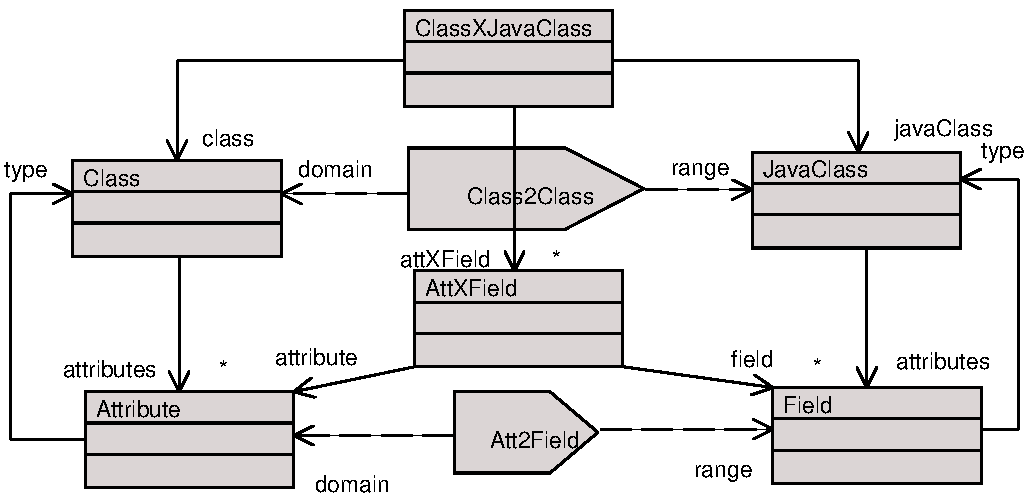
\includegraphics[width=12cm]{Mappings/figures/mappingspec.pdf}
\caption{An example mapping specification} \label{mappingspec}
\end{center}
\end{figure}

OCL is then used to define the constraints on the relationship
between the models. The following constraint requires that the
names of the two classes must be the same.

\begin{lstlisting}
context ClassXJavaClass
  @Constraint SameNames
    class.name = javaClass.name
  end
\end{lstlisting}\noindent This constraint ensures that there is an AttXField
mapping for each attribute owned by a class:

\begin{lstlisting}
context ClassXJavaClass
  @Constraint AttXFieldForClassAtt
    class.attributes = attXField.attribute
  end
\end{lstlisting}\noindent Similar constraints will be required for Java classes.

Mapping specifications are a useful means of validating a mapping.
This can be achieved by firstly specifying the mapping. Next, an
implementation of the mapping is designed so that whenever it is
run it will generate instances of the appropriate mapping
specification classes. The constraints on the mapping
specification can then checked to test that the mapping
implementation has satisfied the mapping specification.

\section{Mapping Issues}

\subsection{Merging}

The previous example highlights an important issue that often
occurs when writing mappings: how to merge duplicate elements.
Duplicate elements typically occur when mapping graph like
structures. Elements in the graph may have references to other
elements in the graph that have already been mapped. In this
situation, naively following the link and mapping the element will
result in duplicate elements being generated.

A good example is a mapping between UML and Java (a simplified
model is shown in figure \ref{umlmapping}). One way to implement
this mapping is to traverse each of the classes in the package,
and then map each class and its associated attributes to Java
classes and fields. A problem arises because Java classes
reference their types (thus introducing a circular dependency). At
the point at which a Att2Field mapping is executed, the generated
Field's type may already have been generated. If the Att2Field
mapping then generates a new type, it will be duplicated.

\begin{figure}[htb]
\begin{center}
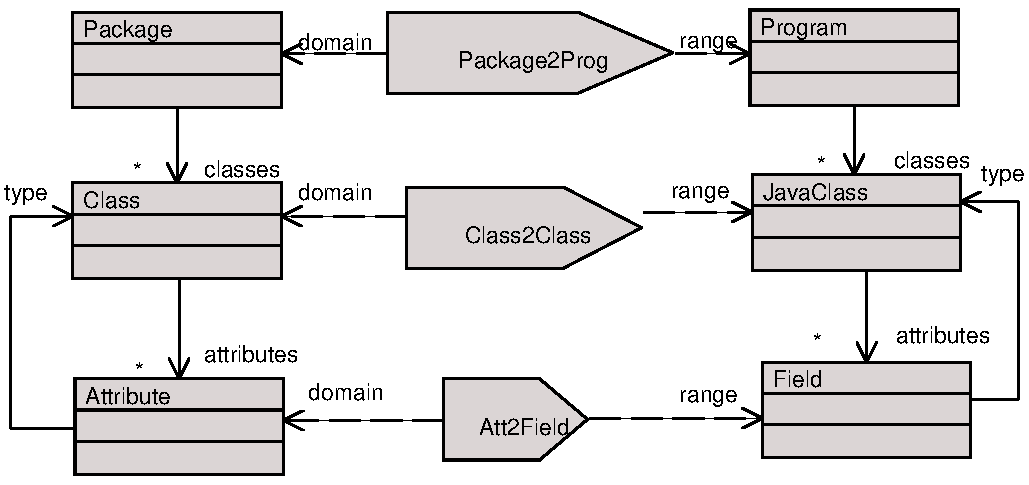
\includegraphics[width=12cm]{Mappings/figures/umlmapping.pdf}
\caption{A simplified UML to Java mapping} \label{umlmapping}
\end{center}
\end{figure}

\noindent There are a number of solutions to this problem:

\begin{itemize}
\item Maintain a table of generated elements and check it before
generating a new element. The Java to XML mapping described above
is an example of this. \item Run the mapping and then merge
duplicate elements on a case by case basis. An example of how this
is achieved in XOCL can be found in section \ref{merge}. \item Use
a generic mechanism that can run over object graphs merging
duplicate elements. The walker algorithm defined in section
\ref{walker} can form the basis for such an algorithm.
\end{itemize}

In all cases, criteria must be identified for mergeable elements.
In above mapping, the criteria for merging two types is that they
have the same name. In general, the criteria must be defined on a
case by case basis, and accommodated in the mappings.

\subsection{Traceability}

A common requirement when constructing mappings is to keep
information about the mapping. There are two strategies that can
be used to achieve this:

\begin{itemize}
\item Create instances of reverse mappings or mapping
specifications as the mapping is performed. The result will be a
graph of reverse mappings or mapping specifications connecting the
domain and range elements. \item Extend the mapping language so
that it records a trace of the executed mappings in a generic.
\end{itemize}

The former approach is most appropriate when wishing to reverse
the mapping or check that it satisfies a specification of the
mapping. The latter approach is most useful when analysing or
debugging a mapping.

\section{XSync}

Very often mappings are required that are not uni-directional, but
which synchronise elements, ensuring that if changes occur in one
element they are reflected in another. There are many applications
of synchronised mappings, including:

\begin{itemize}
\item Maintaining consistency between views on a common collection
of elements: for instance, keeping diagrams consistent with models
and vice versa. \item Managing multiple models of a system: for
example, a large systems development project might use multiple
tools to design different aspects of a system but be required to
maintain consistency where design data overlaps. \item Supporting
round trip engineering where models are maintained in sync with
code and vice versa.
\end{itemize}

XSync is a mapping language that permits the modelling of
synchronised mappings. It enables rules about the relationship
between concepts in two or more models to be captured at a high
level of abstraction. Synchronised mappings can be run
concurrently, continuously monitoring and managing relationship
between elements.

\subsection{Examples}

The following code describes a simple XSync model in which we want
to maintain consistency between two instances of a class. The
class is defined as follows:

\begin{lstlisting}
context Root
  @Class Point
    @Attribute x : Integer end
    @Attribute y : Integer end
    @Constructor(x,y) ! end
  end
\end{lstlisting}\noindent We create two instances of the class, p1 and p2:

\begin{lstlisting}
Root::p1 := Point(100,100); Root::p2 := Point(1,2);
\end{lstlisting}\noindent Now we create a synchronised mapping:

\begin{lstlisting}
Root::n1 :=

@XSync
  @Scope
    Set{p1,p2}
  end
  @Rule r1 1
      p1 = Point[x=x;y=y];
      p2 = Point[x=x;y=y] when p1 <> p2
    do
      "The points match".println()
  end
  @Rule r2 1
      p1 = Point[x=x1];
      p2 = Point[x=x2] when p1 <> p2 and x1 < x2
    do
      "Incrementing x".println();
      p1.x := x1 + 1
  end
  @Rule r3 1
      p1 = Point[y=y1];
      p2 = Point[y=y2] when p1 <> p2 and y1 < y2
    do
      "Incrementing y".println();
      p1.y := y1 + 1
  end
end;
\end{lstlisting}A synchronised mapping consists of a scope and a collection of
synchronisation rules. The scope of the mapping is the collection
of elements over which the mapping applies. In this case, it is
the two instances of Point, p1 and p2.

A rule describes the condition under which an action should occur.
Actions are used to describe synchronisations but they may also
cause other side effects. This is important because in practice it
is often necessary to perform other tasks such as generating
reports, modifying values and so on.

A rule takes the form of a pattern, a boolean 'when' clause and a
'do' action. Provided that the 'when' clause is satisfied by
variables introduced by a matched pattern, the 'do' action will be
invoked.

In this example, rule r1 checks to see whether p1 and p2 match
against instances of Point that have the same x and y values. If
they do, and  p1 and p2 are not the same element, the 'do' action
is invoked to display a message. Rule r2 matches the x values of
p1 and p2 against the variables x1 and x2. If x1 is less than x2,
the value of p1's x is incremented. Rule r3 does the same for the
y values. The result of running this mapping with two points with
different x or y values will be to increment the values until they
are synchronised.

The previous example is limited as it is fixed to two specific
instances. The following shows how a synchronisation mapping can
be parameterised by an operation:

\begin{lstlisting}
context Root
  @Operation sameName(c1,c2)
    @XSync
      @Scope
        Set{c1,c2}
      end
      @Rule r1 1
        x1 = Class[name = n1] when x1 = c1;
        x2 = Class[name = n2] when x2 = c2 and n1 <> n2
        do x1.name := x2.name
      end
    end
  end
\end{lstlisting}This mapping applies to any pair of classes and synchronises the
name of the first with the second. Such a mapping would be useful
for synchronising concrete syntax classes and abstract syntax
classes, for example see chapter \ref{concretechapter}.

This section has provided a short introduction to the XSync
synchronisation language. Future versions of this book will
explore a number of deeper issues, including its application to
the synchronisation of complex structures, and the different
execution models it supports.

\section{Conclusion}

Mappings are a central part of Language-Driven Development as they
enable key relationships between many different types of problem
domain to be captured. Mappings exist between vertical, horizontal
and variant dimensions of a problem domain. In the context of
languages, mappings are needed to synchronise abstract and
concrete syntaxes and to relate models and programs written in
different languages.
